\documentclass[portrait,a0paper,fontscale=0.4]{baposter}

% Packages for input encoding and localization
\usepackage[utf8]{inputenc}
\usepackage[english]{babel}

\usepackage[font=small,labelfont=bf]{caption}
\usepackage{float}
\usepackage{relsize} % http://ftp.gwdg.de/pub/ctan/macros/latex/contrib/relsize/relsize-doc.pdf
\usepackage{tcolorbox}
\usepackage{textcomp}

\definecolor{azure}{rgb}{0.0, 0.5, 1.0}
\definecolor{babyblueeyes}{rgb}{0.63, 0.79, 0.95}
\definecolor{blue-violet}{rgb}{0.54, 0.17, 0.89}
% Package for better URL support
\usepackage{url}

% Package to include graphics
\usepackage{graphicx}
\graphicspath{{./fig/}}
\DeclareGraphicsExtensions{.png,.pdf,.jpg,.jpeg}
\usepackage{subfig}
\usepackage{enumitem}

\setlength{\abovecaptionskip}{-5pt}

\usepackage{palatino}
% Package for program listings
\usepackage{listings}
% Settings for the listings package
\lstset{
  language=C,
  emphstyle={\em},
  }

% Packages for nicer tables
\usepackage{tabularx}
\usepackage{multirow}
\usepackage{booktabs} % for tables
\captionsetup[figure]{labelformat=simple,skip=0.75em,name=Fig.}

\newcommand{\tabularTextSize}[0]{\tiny}

\newcommand{\mycomment}[1]{}



\newcommand{\verytiny}{\fontsize{4}{12} \selectfont \setlength{\baselineskip}{4pt plus 2pt minus 1pt}}

% Save space in lists. Use this after the opening of the list
\newcommand{\compresslist}{%
\setlength{\itemsep}{1pt}%
\setlength{\parskip}{0pt}%
\setlength{\parsep}{0pt}%
}


\begin{document}

  \definecolor{UHAM}{HTML}{e30613} %87CEEB
  \definecolor{UHAMLight}{HTML}{e37673} %87CEEB


  % % Setting the watermark image
  % \background
  % {
  %     \begin{tikzpicture}[remember picture,overlay]%
  %     \draw (current page.center) node[opacity=0.3]
  %       {\includegraphics[scale=5]{SIOX-Logo}};
  %     \end{tikzpicture}%
  % }

\begin{poster}
{ % key=value option
  grid=false,
  columns = 4,
  eyecatcher=true,
  background=shadeTB,%user
  bgColorOne=white,
  bgColorTwo=white,
  borderColor=UHAM,
  headerColorOne=UHAMLight,
  headerColorTwo=UHAMLight,%white
  headershape=rounded,
  headerheight=4.8cm,
  textfont={\setlength{\parindent}{0em} \setlength{\parskip}{0.75em}},
  headerborder=open,
  textborder=rounded,
  boxshade=plain,%shadeTB
  boxColorOne=white,
  boxColorTwo=UHAM
}{ % Eye Catcher
  %
}{ % Poster Title
  \textbf{The Virtual Institute for I/O and the IO-500}
  %\medskip
  %\textbf{\huge xx}
}{ % Poster Authors
  \vspace{0.5em}
  \textsc
  Julian Kunkel$^1$, Jay Lofstead$^2$, John Bent$^3$
  \\[0.5em]
  \emph{$^1$ Deutsches Klimarechenzentrum (DKRZ)}
  \hspace*{2em}
  \emph{$^2$ Sandia National Laboratory}
   \hspace*{2em}
  \emph{$^3$ Seagate}
  \\[0.5em]
   Contact: \url{kunkel@dkrz.de}
}{
    \begin{minipage}{0.2\textwidth}
      
\includegraphics[width=\textwidth]{logo-vi4io.png}
    \end{minipage}
}


\begin{posterbox}[name=problem,column=0]
{Introduction}

The research community in high-performance computing is organized loosely.
There are many distinct resources such as homepages of research groups and benchmarks.
The Virtual Institute for I/O aims to provide a hub for the community and particularly newcomers to find relevant information in many directions.
Additionally, we host the \textbf{high-performance storage list}. Similarly to the top500, it contains information about supercomputers and their storage systems.
Additionally, in the community, we are working on standardizing an I/O benchmark.

This poster introduces the Virtual Institute for I/O, the high-performance storage list and the effort for the IO-500 which are unfunded community projects.
\end{posterbox}


\begin{posterbox}[name=approach,column=0,below=problem]
{The Virtual Institute for I/O}


Goals of the Virtual Institute for I/O (VI4IO) are
\vspace*{-1em}
\begin{itemize}\compresslist
\item Provide a platform for I/O researchers and enthusiasts for exchanging information
\item Foster training and international collaboration in the field of high-performance I/O
\item Track/encourage the deployment of large storage systems by hosting information about high-performance storage systems
\end{itemize}
\vspace*{-1em}

The philosophical cornerstones of VI4IO are:

\vspace*{-1em}
\begin{itemize}\compresslist
\item Treat contributors/participants equally
\item Allow free participation without any fee inclusive to all
\item Independent of vendors/research facilities
\end{itemize}
\end{posterbox}


\begin{posterbox}[name=overview,column=0,below=approach]{Open Organization}

The organization uses a wiki as central hub
\vspace*{-1em}
\begin{itemize}\compresslist
\item Registered users can edit the content
\item Mayor changes should be discussed on the contribute mailing list
\item Tag clouds link between similar entities
\item Supported by mailing lists, e.g.:
\begin{itemize}\compresslist
\item Call-for-papers
\item Announcements
\item Contributions / suggestions
\end{itemize}
\end{itemize}

\end{posterbox}


\begin{posterbox}[name=wps,column=0,above=bottom,below=overview]{HPSL System Model}
The system model describes how characteristics are assigned to components.
Storage is difficulty to assign to a single component as it is often shared across supercomputers,
therefore, a component based model is used.

Supported components:
\vspace*{-1em}
\begin{itemize}\compresslist
\item Site: Describes the facility
\item Supercomputer: A system
\item Storage (shared, local or nearline storage)
\end{itemize}

\vspace*{-1em}

Conceptual example:

\vspace*{-1em}
\begin{center}
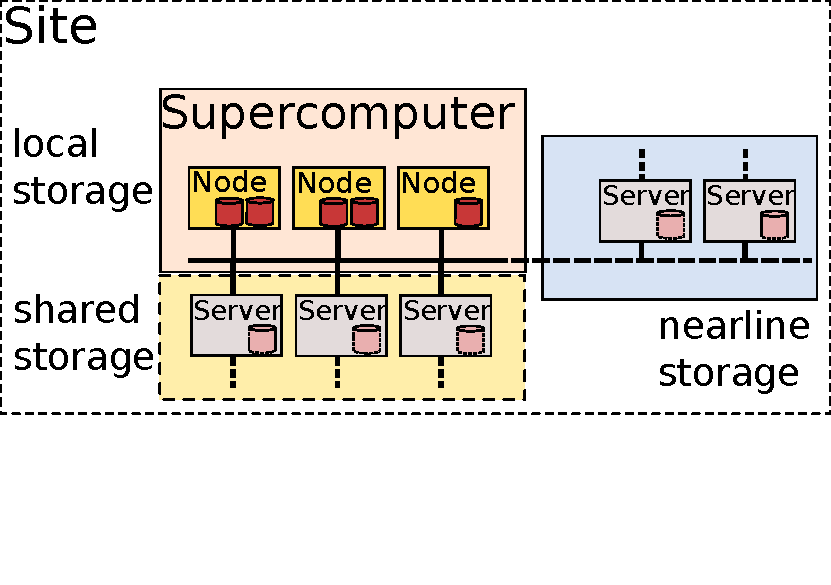
\includegraphics[width=0.9\textwidth]{model}
\end{center}

\vspace*{-5em}

The web page allows the creation of a topology for the facility to indicate the relation between the components.
An example for DKRZ:

\vspace*{-1em}

\begin{center}
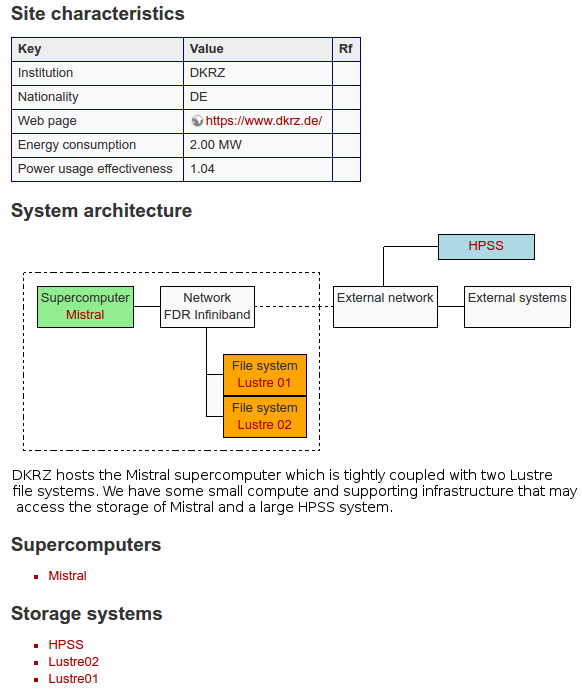
\includegraphics[width=0.95\textwidth]{dkrz-site}
\end{center}

\end{posterbox}



\begin{posterbox}[name=concept,column=1,span=2]{Content of the VI4IO Wiki}


\end{posterbox}


\begin{posterbox}[name=schedule,column=1,span=2, below=concept]{High-Performance Storage List}
Sortable, allows to add/remove columns (see the list next for the menu)

Graphing and individual grouping 

Metrics?
\end{posterbox}

\begin{posterbox}[name=HHCC,column=1,span=2, below=schedule, above=bottom]{IO-500 Effort}
\end{posterbox}




\begin{posterbox}[name=engineering,column=3]{HPSL 2017}
The current list contains 30 supercomputers:
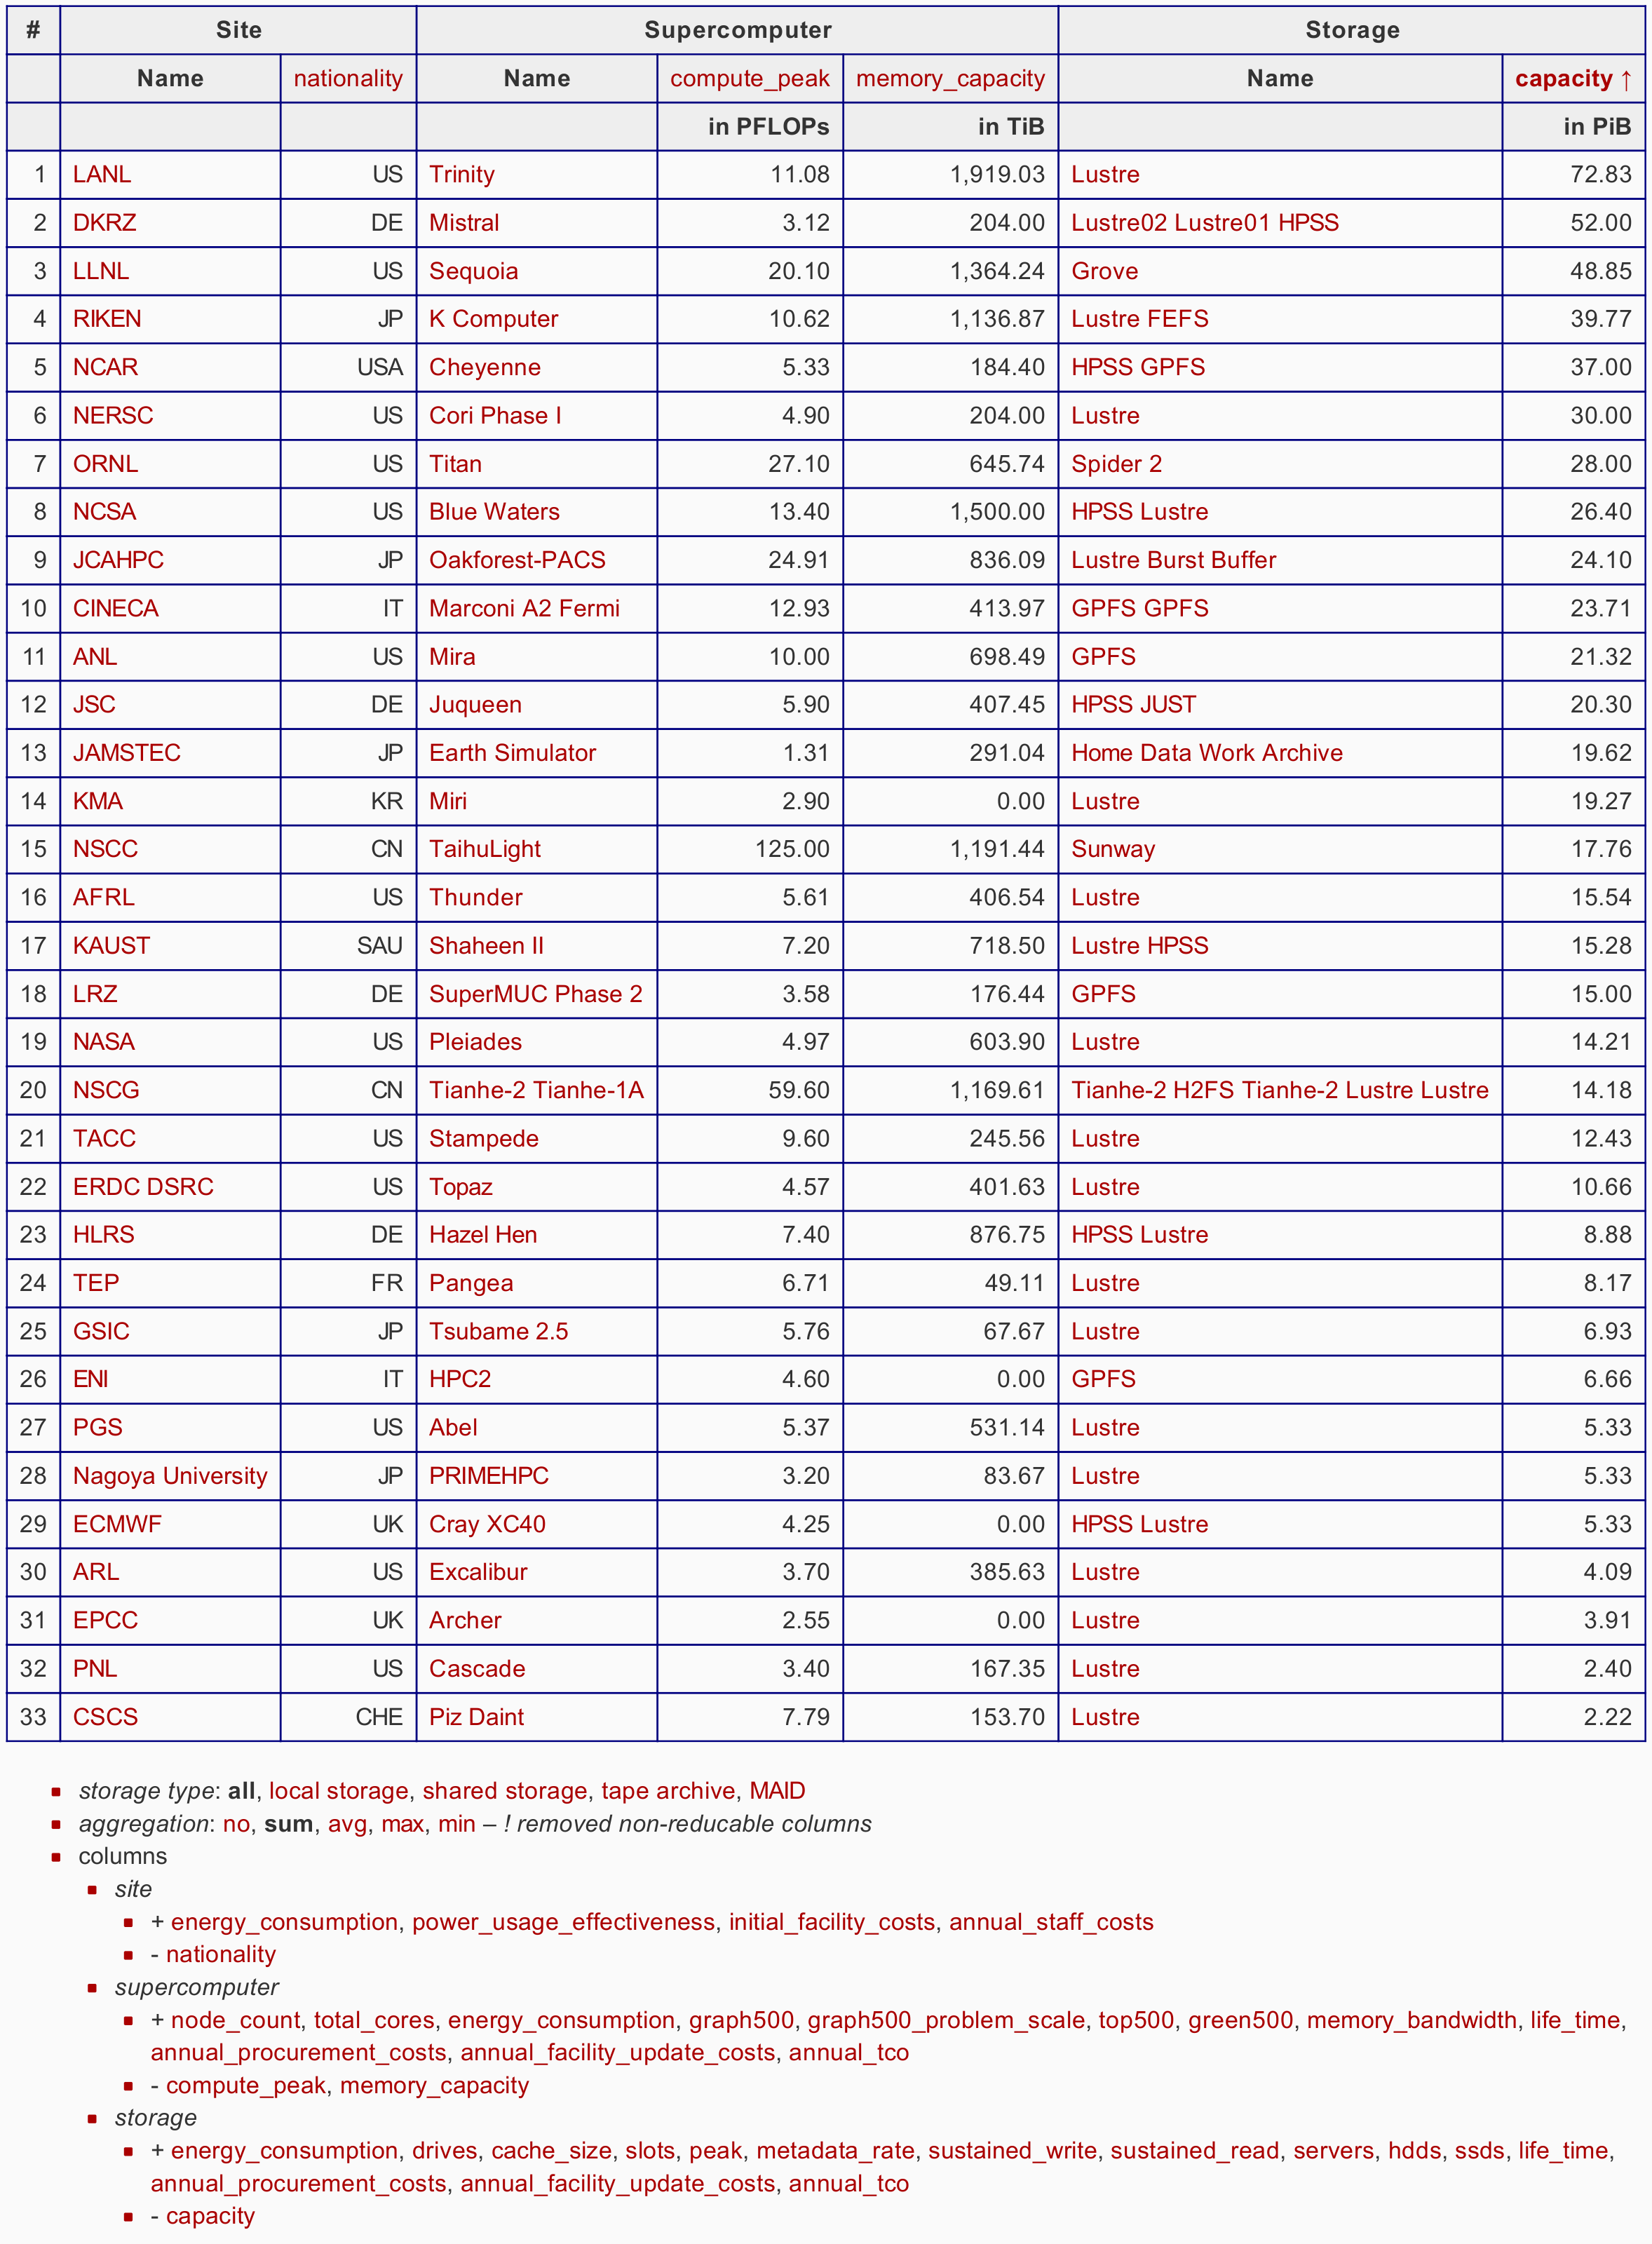
\includegraphics[width=\textwidth]{hpsl-current}

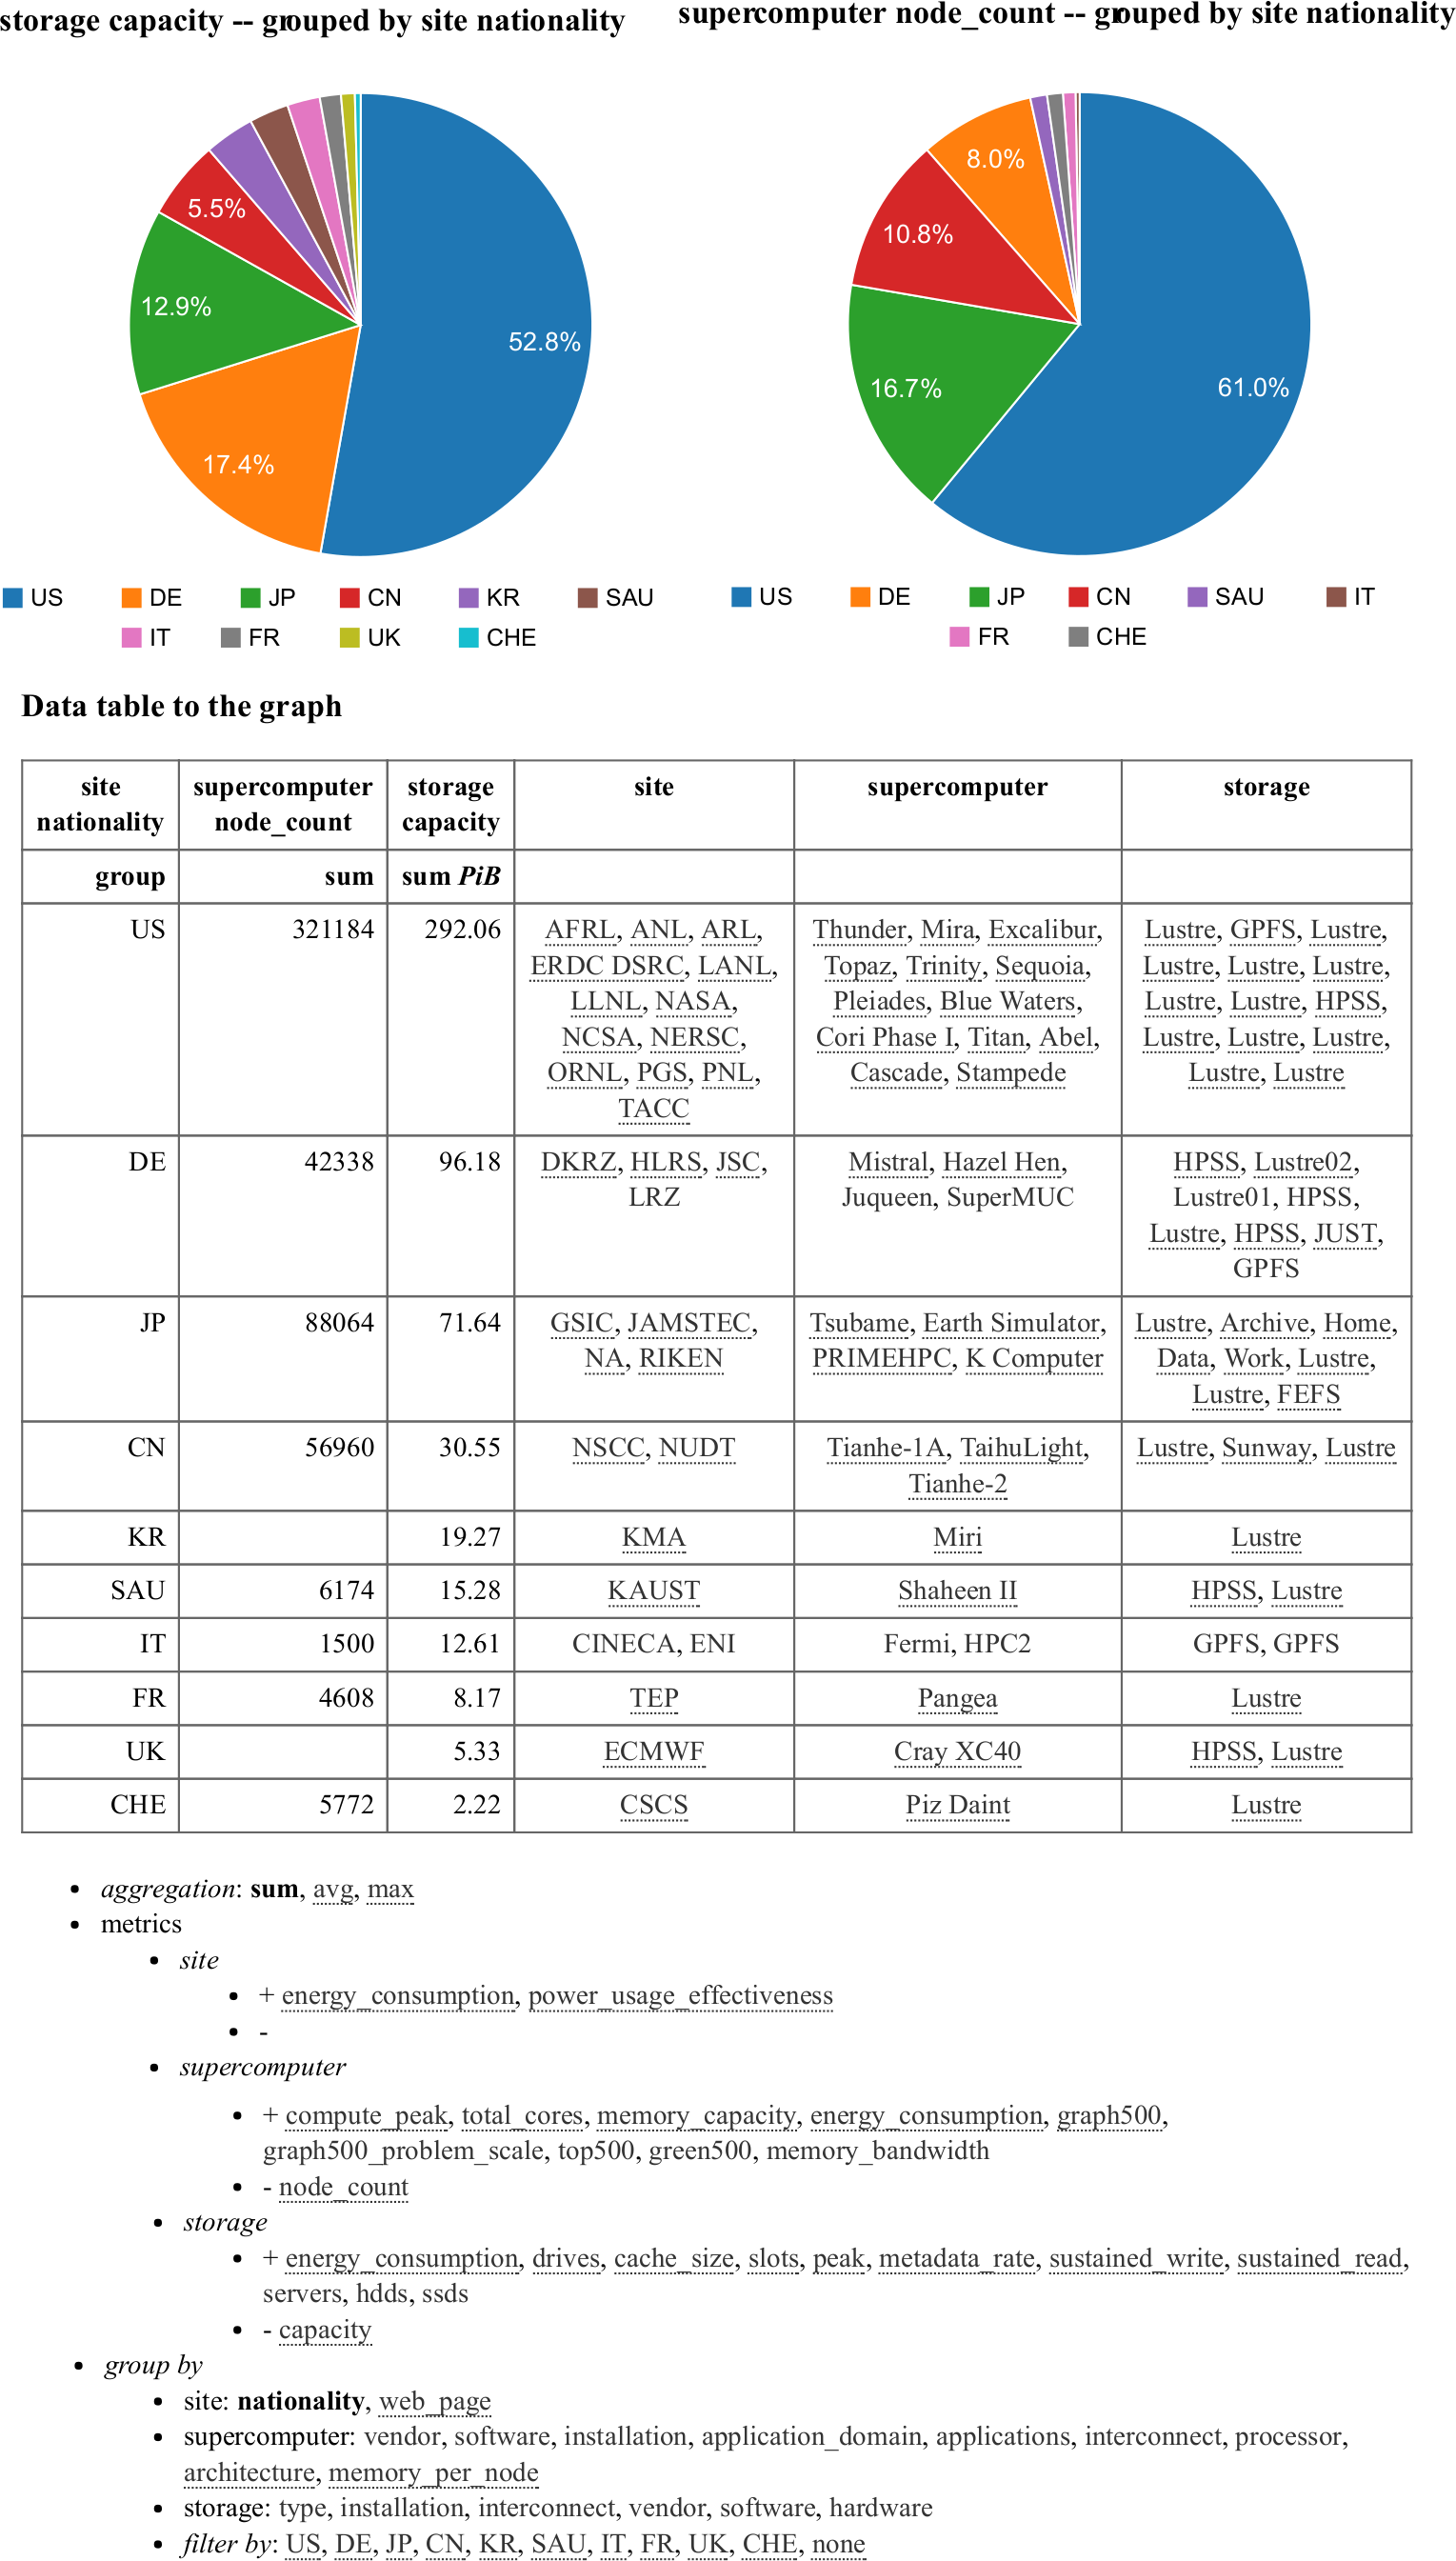
\includegraphics[width=\textwidth]{hpsl-figure}
\end{posterbox}




\begin{posterbox}[name=awareness,column=3,below=engineering]{Derived Analysis}
With the collected data many in-depth analysis becomes possible, for example, 
the relationship between storage and memory capacity:

\vspace*{-1em}

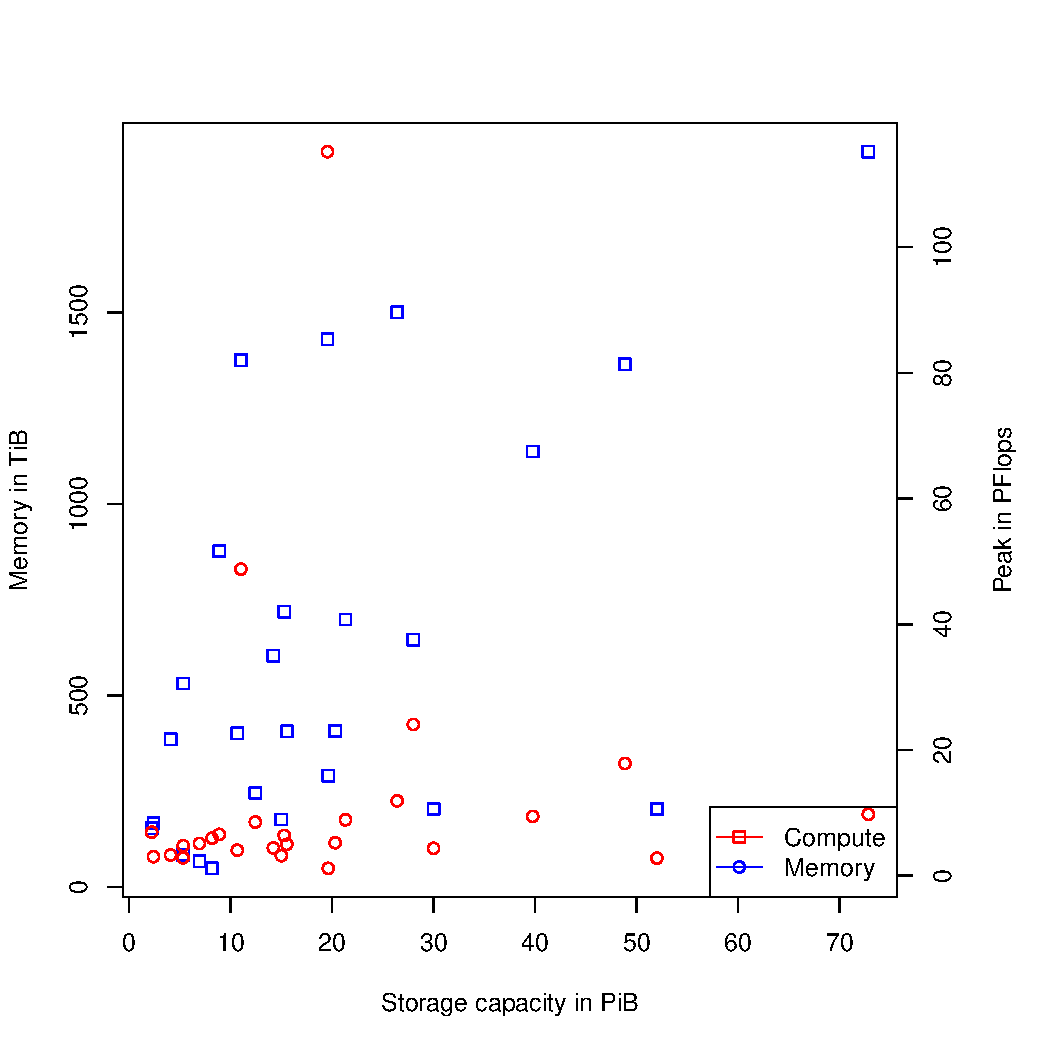
\includegraphics[width=5cm]{capacityvscompute}
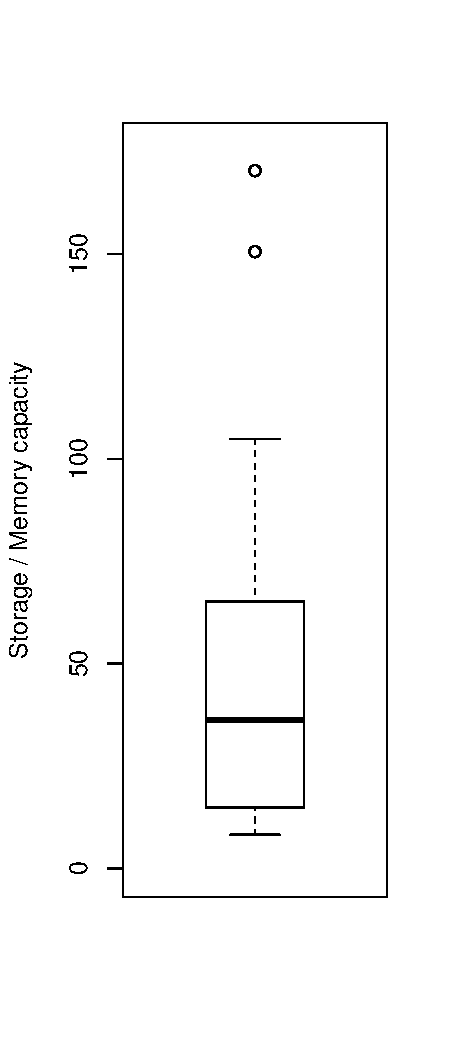
\includegraphics[width=2.15cm]{capacitymemory}

\vspace*{-2em}
\begin{itemize}\compresslist
\item Correlation storage capacity vs.
  \begin{itemize}\compresslist
  \item memory capacity = 0.58      
  \item compute peak = 0.04
  \end{itemize}
\item Mean(storage/mem capacity) = 54.6
\end{itemize}

\end{posterbox}


\begin{posterbox}[name=hpccertification,column=3,below=awareness, above=bottom]{VI4IO and You}
Content is under open licenses. 
You are welcome to join the mailing lists or participate!

\huge \url{https://vi4io.org}
\end{posterbox}


\end{poster}
\end{document}
